% commandes
\newcommand{\notion}[1]{\textcolor{vert_fonce}{\textit{#1}}}
\newcommand{\mb}[1]{\mathbb{#1}}
\newcommand{\mc}[1]{\mathcal{#1}}
\newcommand{\mr}[1]{\mathrm{#1}}
\newcommand{\code}[1]{\texttt{#1}}
\newcommand{\ccode}[1]{\texttt{|#1|}}
\newcommand{\ov}[1]{\overline{#1}}
\newcommand{\abs}[1]{|#1|}
\newcommand{\rev}[1]{\texttt{reverse(#1)}}
\newcommand{\crev}[1]{\texttt{|reverse(#1)|}}

\newcommand{\ie}{\textit{i.e.} }

\newcommand{\N}{\mathbb{N}}
\newcommand{\R}{\mathbb{R}}
\newcommand{\C}{\mathbb{C}}
\newcommand{\K}{\mathbb{K}}
\newcommand{\Z}{\mathbb{Z}}

\newcommand{\A}{\mathcal{A}}
\newcommand{\bigO}{\mathcal{O}}
\renewcommand{\L}{\mathcal{L}}

\newcommand{\rg}[0]{\mathrm{rg}}
\newcommand{\re}[0]{\mathrm{Re}}
\newcommand{\im}[0]{\mathrm{Im}}
\newcommand{\cl}[0]{\mathrm{cl}}
\newcommand{\grad}[0]{\vec{\mathrm{grad}}}
\renewcommand{\div}[0]{\mathrm{div}\,}
\newcommand{\rot}[0]{\vec{\mathrm{rot}}\,}
\newcommand{\vnabla}[0]{\vec{\nabla}}
\renewcommand{\vec}[1]{\overrightarrow{#1}}
\newcommand{\mat}[1]{\mathrm{Mat}_{#1}}
\newcommand{\matrice}[1]{\mathcal{M}_{#1}}
\newcommand{\sgEngendre}[1]{\left\langle #1 \right\rangle}
\newcommand{\gpquotient}[1]{\mathbb{Z} / #1\mathbb{Z}}
\newcommand{\norme}[1]{||#1||}
\renewcommand{\d}[1]{\,\mathrm{d}#1}
\newcommand{\adh}[1]{\overline{#1}}
\newcommand{\intint}[2]{\llbracket #1 ,\, #2 \rrbracket}
\newcommand{\seg}[2]{[#1\, ; \, #2]}
\newcommand{\scal}[2]{( #1 | #2 )}
\newcommand{\distance}[2]{\mathrm{d}(#1,\,#2)}
\newcommand{\inte}[2]{\int_{#1}^{#2}}
\newcommand{\somme}[2]{\sum_{#1}^{#2}}
\newcommand{\deriveref}[4]{\biggl( \frac{\text{d}^{#1}#2}{\text{d}#3^{#1}} \biggr)_{#4}}





\documentclass{article}
\usepackage{amsmath,amssymb,mathtools}
\usepackage{xcolor}
\usepackage{enumitem}
\usepackage{multicol}
\usepackage{changepage}
\usepackage{stmaryrd}
\usepackage{graphicx}
\usepackage[framemethod=tikz]{mdframed}
\usepackage{tikz,pgfplots}
\pgfplotsset{compat=1.18}

% physique
\definecolor{oranges}{RGB}{255, 242, 230}
\definecolor{rouges}{RGB}{255, 230, 230}
\definecolor{rose}{RGB}{255, 204, 204}

% maths - info
\definecolor{rouge_fonce}{RGB}{204, 0, 0}
\definecolor{bleu_fonce}{RGB}{0, 0, 255}
\definecolor{vert_fonce}{RGB}{0, 69, 33}

\definecolor{orange_foncee}{RGB}{255, 153, 0}
\definecolor{myrtille}{RGB}{225, 225, 255}
\definecolor{mayonnaise}{RGB}{255, 253, 233}
\definecolor{magenta}{RGB}{224, 209, 240}
\definecolor{pomme}{RGB}{204, 255, 204}
\definecolor{mauve}{RGB}{255, 230, 255}


% Cours

\newmdenv[
  nobreak=true,
  topline=true,
  bottomline=true,
  rightline=true,
  leftline=true,
  linewidth=0.5pt,
  linecolor=black,
  backgroundcolor=mayonnaise,
  innerleftmargin=10pt,
  innerrightmargin=10pt,
  innertopmargin=10pt,
  innerbottommargin=10pt,
  skipabove=\topsep,
  skipbelow=\topsep,
]{boite_definition}

\newmdenv[
  nobreak=true,
  topline=true,
  bottomline=true,
  rightline=true,
  leftline=true,
  linewidth=0.5pt,
  linecolor=white,
  backgroundcolor=white,
  innerleftmargin=10pt,
  innerrightmargin=10pt,
  innertopmargin=10pt,
  innerbottommargin=10pt,
  skipabove=\topsep,
  skipbelow=\topsep,
]{boite_exemple}

\newmdenv[
  nobreak=true,
  topline=true,
  bottomline=true,
  rightline=true,
  leftline=true,
  linewidth=0.5pt,
  linecolor=black,
  backgroundcolor=magenta,
  innerleftmargin=10pt,
  innerrightmargin=10pt,
  innertopmargin=10pt,
  innerbottommargin=10pt,
  skipabove=\topsep,
  skipbelow=\topsep,
]{boite_proposition}

\newmdenv[
  nobreak=true,
  topline=true,
  bottomline=true,
  rightline=true,
  leftline=true,
  linewidth=0.5pt,
  linecolor=black,
  backgroundcolor=white,
  innerleftmargin=10pt,
  innerrightmargin=10pt,
  innertopmargin=10pt,
  innerbottommargin=10pt,
  skipabove=\topsep,
  skipbelow=\topsep,
]{boite_demonstration}

\newmdenv[
  nobreak=true,
  topline=true,
  bottomline=true,
  rightline=true,
  leftline=true,
  linewidth=0.5pt,
  linecolor=white,
  backgroundcolor=white,
  innerleftmargin=10pt,
  innerrightmargin=10pt,
  innertopmargin=10pt,
  innerbottommargin=10pt,
  skipabove=\topsep,
  skipbelow=\topsep,
]{boite_remarque}


\newenvironment{definition}[2]
{
    \begin{boite_definition}
    \textbf{\textcolor{rouge_fonce}{Définition #1}} \textit{#2} \\ \\
}
{
    \end{boite_definition}
    \vspace{15pt}
}

\newenvironment{exemple}[2]
{
    \begin{boite_exemple}
    \textbf{\textcolor{bleu_fonce}{Exemple #1}} \textit{#2} \\
    \begin{itemize}[label=$\blacktriangleright \quad $]                    
}
{   
    \end{itemize}
    \end{boite_exemple}
    \vspace{15pt}
}

\newenvironment{proposition}[2]
{
    \begin{boite_proposition}
    \textbf{\textcolor{rouge_fonce}{Proposition #1}} \textit{#2} \\ \\
}
{
    \end{boite_proposition}
    \vspace{15pt}
}

\newenvironment{theoreme}[2]
{
    \begin{boite_proposition}
    \textbf{\textcolor{rouge_fonce}{Théorème #1}} \textit{#2} \\ \\
}
{
    \end{boite_proposition}
    \vspace{15pt}
}

\newenvironment{demonstration}
{
    \begin{boite_demonstration}
    \textbf{\textcolor{rouge_fonce}{Démonstration}}\\ \\
}
{
    \end{boite_demonstration}
    \vspace{15pt}
}

\newenvironment{remarque}[2]
{
    \begin{boite_remarque}
    \textbf{\textcolor{bleu_fonce}{Remarque #1}}\textit{#2} \\ \\
    \begin{itemize}[label=$\blacktriangleright \quad $ ]                    
}
{   
    \end{itemize}
    \end{boite_remarque}
    \vspace{15pt}
}



%Corrections
\newmdenv[
  nobreak=true,
  topline=true,
  bottomline=true,
  rightline=true,
  leftline=true,
  linewidth=0.5pt,
  linecolor=black,
  backgroundcolor=mayonnaise,
  innerleftmargin=10pt,
  innerrightmargin=10pt,
  innertopmargin=10pt,
  innerbottommargin=10pt,
  skipabove=\topsep,
  skipbelow=\topsep,
]{boite_question}



\newenvironment{question}[2]
{
    \begin{boite_question}
    \textbf{\textcolor{rouge_fonce}{Question #1}} \textit{#2} \\ \\
}
{
    \end{boite_question}
    \vspace{15pt}
}

\newenvironment{enumeratebf}{
    \begin{enumerate}[label=\textbf{\arabic*.}]
}
{
    \end{enumerate}
}

\begin{document}
\begin{adjustwidth}{-3cm}{-3cm}


	\centering
	{\LARGE \textsc{Cours de Physique}\par}
	\vspace{1cm}
	{\Large \textsc{TP 16}\par}
	\vspace{1.5cm}
	{\huge\bfseries Résonance du circuit RLC série\par}
	\vspace{2cm}
	{\Large\itshape Raphaël Jontef \& Romain Van Pradelles de Palmaert\par}
	

	\vspace{8cm}


\begin{question}{1}{ - facteur qualité, pulsation, fréquence, période propres}
    Nous avons calculé : \\ \\
    \begin{cases}
        &\omega_0 = 1,4 \times 10^4 \text{ rad} \cdot \text{ s }^{-1} \\
        &f_0 = 2,25 \text{ kHz} \\
        &T_0 = 444 \text{ {$\mu$}s} \\
        &Q = 2,8
    \end{cases}
\end{question}

\begin{question}{2}{ - Lien entre $u_R$ et $i$}
    \begin{center}
        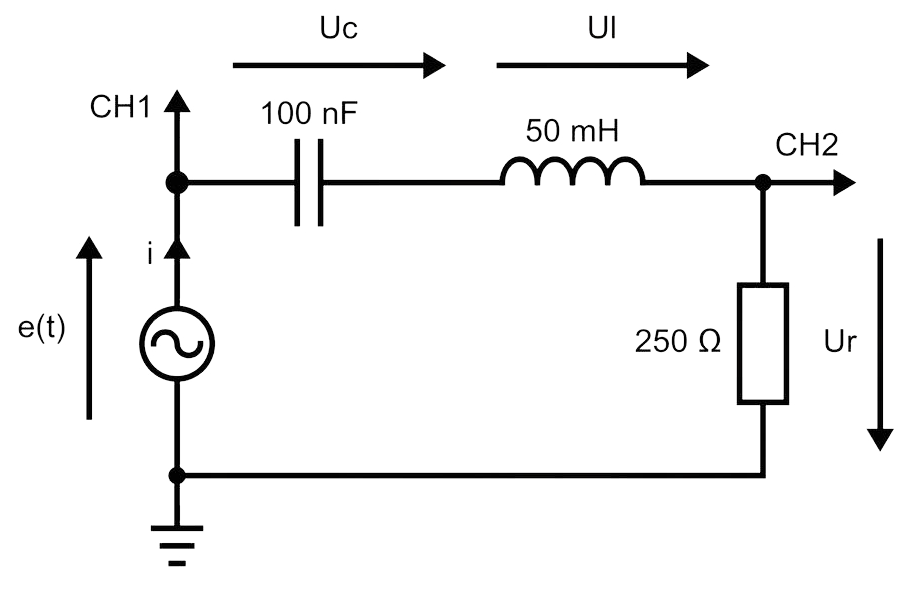
\includegraphics[width=0.4\textwidth]{RLC.png}
    \end{center}
    Par loi d'Ohm, on a \begin{align*}
        &\forall t, u_R(t) = R \cdot i(t)\\
        \implies \Aboxed{&\forall t, i(t) = \frac{u_R(t)}{R}}
    \end{align*}
    $u_R$ et $i$ diffèrent d'une constante multiplicative, leur allure sera donc la même, celle d'une fonction sinusoïdale :
    \begin{center}
        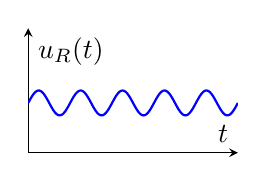
\begin{tikzpicture}
            \begin{axis}[
                width = 0.35\textwidth, height = 90pt,
                xmax = 1800,
                xmin = 0,
                ymax = 10,
                ymin = 0,
                samples=150,
                xtick ={0},
                ytick ={0},
                xlabel={$t$},
                ylabel={$u_R(t)$},
                axis lines=middle,
                grid=major,
                ]
                \addplot[blue,thick,domain=0:1800] {sin(x)+4};
            \end{axis}
        \end{tikzpicture}
    \end{center}
    
    
\end{question}

\begin{question}{3}{ - fréquence de résonance par tâtonnement}
    Cette fréquence $f_r$ vérifie $f_r \approx f_0 = 2,25 \text{ kHz} $.
\end{question}

\begin{question}{4}{ - Application du modèle de Thévenin}
    On modélise le GBF par l'association en série d'une source de tension sinusoïdale idéale avec une résistance $R_g$ de 50 ohms.
    \begin{center}
        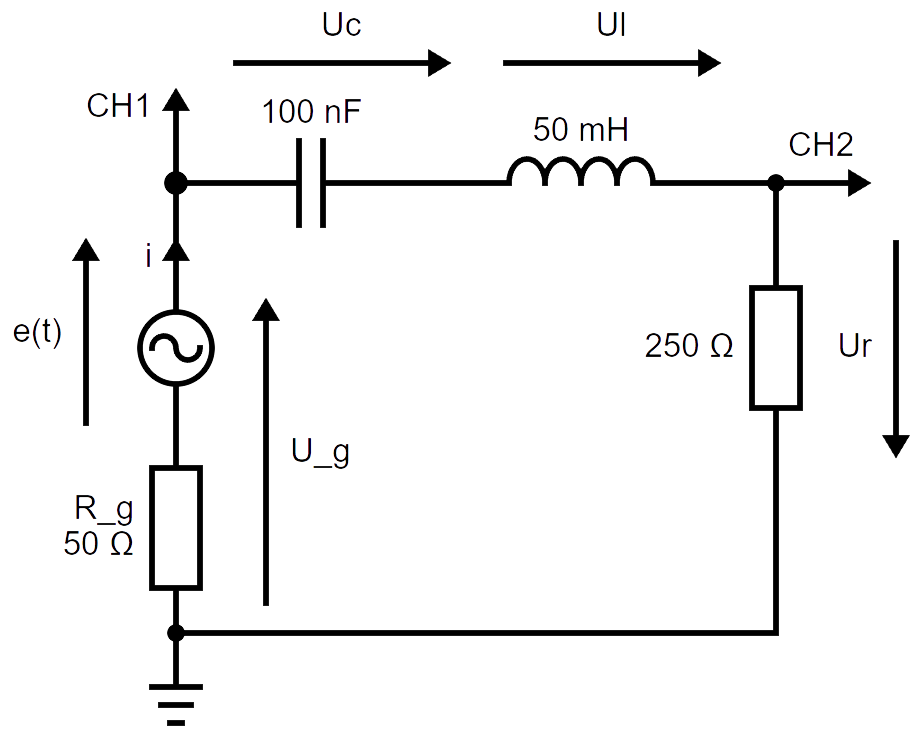
\includegraphics[width=0.4\textwidth]{RRLC.png}
    \end{center}
    À présent, la tension $u_g$ vaut :
       $$\Aboxed{u_g = e(t) - R_g \cdot i(t)} \quad \text{(résistance en convention générateur)}$$
\end{question}

\begin{question}{5}{ - Au voisinage de $f_r$}
    Puisque l'amplitude de $u_g$ est maximale en $f_r$, en s'éloignant de cette fréquence, l'amplitude diminuera.
\end{question}

\begin{question}{6}{ - Mode $XY$}
    \begin{array}{rr}
        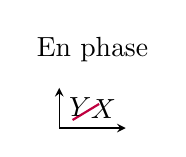
\begin{tikzpicture}
            \begin{axis}[
                width = 0.2\textwidth,
                title = {En phase},
                xmax = 5,
                xmin = 0,
                ymax = 5,
                ymin = 0,
                ytick = {0},
                xtick = {0},
                samples=2,
                xlabel={$X$},
                ylabel={$Y$},
                axis lines=middle,
                grid=major,
                ]
                \addplot[purple,thick,domain =1:3] {x};
            \end{axis}
        \end{tikzpicture} &
        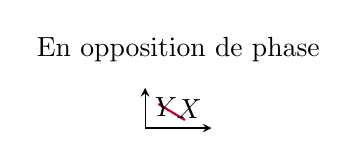
\begin{tikzpicture}
            \begin{axis}[
                width = 0.2\textwidth,
                title = {En opposition de phase},
                xmax = 5,
                xmin = 0,
                ymax = 5,
                ymin = 0,
                ytick = {0},
                xtick = {0},
                samples=2,
                xlabel={$X$},
                ylabel={$Y$},
                axis lines=middle,
                grid=major,
                ]
                \addplot[purple,thick,domain =1:3] {-x + 4};
            \end{axis}
        \end{tikzpicture}
    \end{array}
\end{question}

\begin{question}{7}{ - fréquence de résonance par mode $XY$}
    On adapte la fréquence de $e(t)$ de sorte que $u_R$ (et donc $i$) soit en phase avec $u_g$.
\end{question}

\begin{question}{9}{ - Graphe de $G = \frac{U_R}{U_g}$}
    \begin{center}
        \begin{tikzpicture}
            \begin{axis}[
            ,axis x line=bottom,axis y line=left
            ,xmin=0,xmax=6.24
            ,ymin=0,ymax=0.8805
            ,grid=major
            ,title={Graphe ajusté de $\displaystyle G(f) = \frac{U_R}{U_g}$}
            ,xlabel={$f$/kHz}
            ,ylabel={$G$}
            ]
            \addplot[draw=black,only marks,mark=*,mark options={fill=black}] file {../Presentation/courbes/G10.txt};
            \addplot[draw=blue,mark=none,smooth] file {../Presentation/courbes/G11.txt};
            \addplot[draw=black,only marks,mark=*,mark options={fill=black}] file {../Presentation/courbes/G12.txt};

            \addplot[black,dashed,domain=0:6.5] {0.5982} node [pos=0.8,above right,text=black]{$\displaystyle \frac{G_{max}}{\sqrt{2}}$};
            \draw[vert_fonce] (axis cs:1.884,\pgfkeysvalueof{/pgfplots/ymin}) -- (axis cs:1.884,0.5982) node [pos=0.135,below left]{$f_{c1}$};
            \draw[vert_fonce] (axis cs:2.687,\pgfkeysvalueof{/pgfplots/ymin}) -- (axis cs:2.687,0.5982) node [pos=0.135,below right]{$f_{c2}$};
            \end{axis}
        \end{tikzpicture}
        \end{center}
\end{question}


\begin{question}{10}{ - Déterminaison de $Q$}
    Nous trouvons : 
    \begin{cases}
        &f_{c1} = 1,884 \text{ kHz} \\
        &f_{c2} = 2,687 \text{ kHz}
    \end{cases} \\
    En prenant, $f_r$ = $2225$ Hz, on obtient $\Aboxed{Q = 2.802}$. C'est tout à fait satisfaisant.
\end{question}

\begin{question}{11}{ - Graphe de $\varphi_{R/g}$}
    \begin{center}
        \begin{tikzpicture}
            \begin{axis}[
            ,axis x line=bottom,axis y line=left
            ,xmin=0,xmax=6.24
            ,ymin=-1.49,ymax=1.507
            ,grid=major
            ,title={Graphe ajusté de $\varphi_{R/g}$}
            ,xlabel={$f$/kHz}
            ,ylabel={$\varphi_{R/g}$/rad}
            ]
            \addplot[draw=black,only marks,mark=*,mark options={fill=black}] file {../Presentation/courbes/varphi10.txt};
            \addplot[draw=blue,mark=none,smooth] file {../Presentation/courbes/varphi11.txt};
            \addplot[draw=black,only marks,mark=*,mark options={fill=black}] file {../Presentation/courbes/varphi12.txt};
            \end{axis}
        \end{tikzpicture}
    \end{center}
\end{question}

\end{adjustwidth}
\end{document}